\documentclass[12pt, addpoints]{exam}
\usepackage[left=0.1in, right=0.1in, top=0.6in,bottom=0.1in]{geometry}
\usepackage{enumitem}
\usepackage{amsmath}
\usepackage{tikz}
\usepackage{ulem}
\usetikzlibrary{shapes.geometric, arrows.meta, positioning}

% --- Tikz set for diagram
\tikzset{
    box/.style={rectangle, draw, minimum width=1.8cm, minimum height=1cm, align=left, font=\small},
    doublebox/.style={rectangle, draw, double, double distance=1.5pt, minimum width=2.5cm, minimum height=1cm, align=left, font=\small},
    decision/.style={diamond, draw, minimum width=1cm, minimum height=1cm, align=center, aspect=2, font=\small},
    doubledecision/.style={diamond, double, draw, minimum width=1cm, minimum height=1cm, align=center, aspect=2, font=\small},
    attribute/.style={rectangle, draw, minimum width=1.5cm, minimum height=0.6cm, align=center, font=\small},
    arrow/.style={-Stealth, thick},
    doublearrow/.style={-Stealth, thick, double, double distance=1.5pt},
    dashedline/.style={thick, dashed},
    line/.style={thick},
    doubleline/.style={thick, double, double distance=1.5pt}
}

% --- Make choices use open circles instead of letters ---
\renewcommand{\choicelabel}{\raisebox{0.15ex}{$\bigcirc$}}


% Header/footer formatting
\pagestyle{headandfoot}
\runningheadrule
\firstpageheadrule
\firstpageheader{Database Management Systems}{Test 4 Old}{Fall 2025}
\runningheader{}{Test 4 Old}{}
\runningfooter{}{}{}

\begin{document}
\noindent Name:\ \makebox[3in]{\hrulefill}\hfill Points Scored: \underline{\hspace{3em}} / \numpoints
\begin{questions}

% ------------------ TRUE/FALSE SECTION ------------------
\section*{Part I — True/False}

\begin{minipage}{\linewidth}
\question[2]
True or False: An entity is always represented by one table.\par\vspace{0.5em}
\begin{checkboxes}
    \choice True
    \CorrectChoice False
\end{checkboxes}
\begin{solution}
Not if it has multivalued attribute(s).
\end{solution}
\end{minipage}\vspace{1em}

\begin{minipage}{\linewidth}
\question[2]
True or False: If \textbf{f} was a stored function with one parameter of type varchar(20) returning an integer, 
then the following command would work\par\vspace{0.5em}
select \textbf{f}('HelloThere');\par\vspace{0.5em}
\begin{checkboxes}
    \CorrectChoice True
    \choice False
\end{checkboxes}
\end{minipage}\vspace{1em}

\begin{minipage}{\linewidth}
\question[2]
True or False: Below is the DDL command creating table prereq in the University database.\par
In this definition, there is no "on delete cascade" on an attribute prereq\_id. 
Two triggers are needed in order to ensure that any tuple can be deleted from the University database.\par\vspace{0.5em}
\begin{verbatim}
create table prereq
(course_id        varchar(8), 
prereq_id        varchar(8),
primary key (course_id, prereq_id),
foreign key (course_id) references course(course_id) on delete cascade,
foreign key (prereq_id) references course(course_id)
);
\end{verbatim}
\begin{checkboxes}
    \choice True
    \CorrectChoice False
\end{checkboxes}
\begin{solution}
One trigger is needed: "delete on section".
\end{solution}
\end{minipage}\vspace{1em}


% ------------------ MULTIPLE CHOICE SECTION ------------------

\section*{Part II — Multiple choice (choose one)}

\begin{minipage}{\linewidth}
\question[4]
How many tables will be created in the database for the model depicted in the below ER Diagram?\par\vspace{1em}
\begin{center}
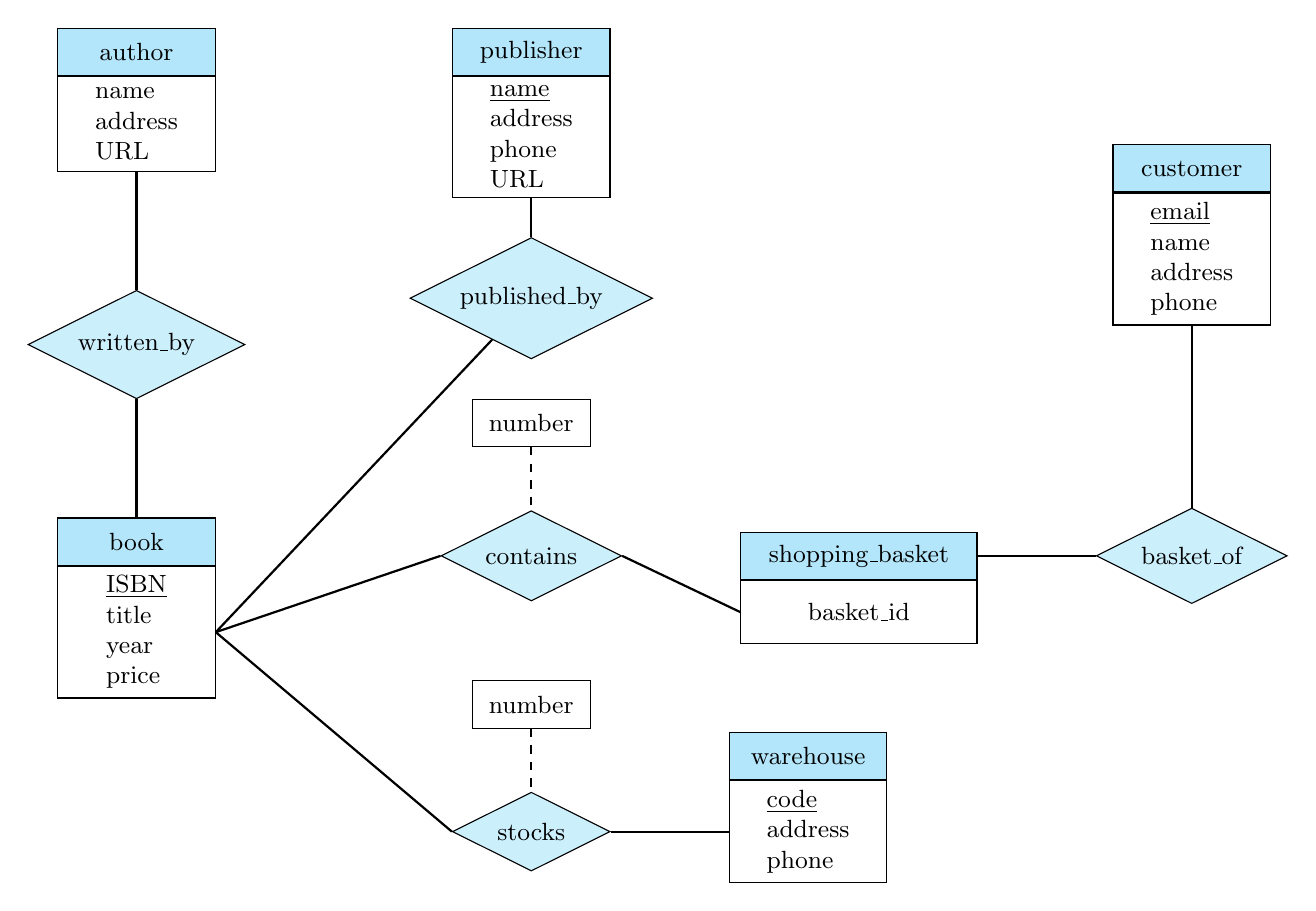
\begin{tikzpicture}[node distance=1.5cm]
    % Author table (top left)
    \node[box, fill=cyan!30, minimum height=0.6cm, minimum width=2cm] (author_header) {author};
    \node[box, fill=white, below=0cm of author_header.south, anchor=north, minimum height=1.2cm, minimum width=2cm] (author_body) {name\\address\\URL};
    
    % Written_by diamond
    \node[decision, below=1.5cm of author_body, fill=cyan!20] (written_by) {written\_by};
    
    % Book table
    \node[box, fill=cyan!30, minimum height=0.6cm, minimum width=2cm, below=1.5cm of written_by] (book_header) {book};
    \node[box, fill=white, below=0cm of book_header.south, anchor=north, minimum height=1.4cm, minimum width=2cm] (book_body) {\underline{ISBN}\\title\\year\\price};
    
    % Publisher table (top center, closer to author)
    \node[box, fill=cyan!30, minimum height=0.6cm, minimum width=2cm, right=3cm of author_header] (publisher_header) {publisher};
    \node[box, fill=white, below=0cm of publisher_header.south, anchor=north, minimum height=1.5cm, minimum width=2cm] (publisher_body) {\underline{name}\\address\\phone\\URL};
    
    % Published_by diamond
    \node[decision, below=0.5cm of publisher_body, fill=cyan!20] (published_by) {published\_by};
    
    % Number attribute for contains (top)
    \node[attribute, below=0.5cm of published_by] (number1) {number};
    
    % Contains diamond
    \node[decision, below=0.8cm of number1, fill=cyan!20] (contains) {contains};
    
    % Shopping_basket table
    \node[box, fill=cyan!30, minimum height=0.6cm, minimum width=3cm, right=1.5cm of contains] (basket_header) {shopping\_basket};
    \node[box, fill=white, below=0cm of basket_header.south, anchor=north, minimum height=0.8cm, minimum width=3cm] (basket_body) {basket\_id};
    
    % Basket_of diamond (next to shopping_basket)
    \node[decision, right=1.5cm of basket_header, fill=cyan!20] (basket_of) {basket\_of};
    
    % Customer table (above basket_of)
    \node[box, fill=cyan!30, minimum height=0.6cm, minimum width=2cm, above=4cm of basket_of] (customer_header) {customer};
    \node[box, fill=white, below=0cm of customer_header.south, anchor=north, minimum height=1.4cm, minimum width=2cm] (customer_body) {\underline{email}\\name\\address\\phone};
    
    % Number attribute for stocks (bottom)
    \node[attribute, below=1cm of contains] (number2) {number};
    
    % Stocks diamond
    \node[decision, below=0.8cm of number2, fill=cyan!20] (stocks) {stocks};
    
    % Warehouse table
    \node[box, fill=white, anchor=north, minimum height=1.2cm, minimum width=2cm, right=1.5cm of stocks] (warehouse_body) {\underline{code}\\address\\phone};
    \node[box, fill=cyan!30, above=0cm of warehouse_body.north, minimum height=0.6cm, minimum width=2cm] (warehouse_header) {warehouse};

    % Lines
    \draw[line] (author_body) -- (written_by);
    \draw[line] (written_by) -- (book_header);
    \draw[line] (publisher_body) -- (published_by);
    \draw[line] (published_by) -- (book_body.east);
    \draw[line] (book_body.east) -- (contains.west);
    \draw[dashedline] (number1) -- (contains);
    \draw[line] (contains.east) -- (basket_body.west);
    \draw[line] (customer_body) -- (basket_of);
    \draw[line] (basket_of) -- (basket_header.east);
    \draw[line] (book_body.east) -- (stocks.west);
    \draw[dashedline] (number2) -- (stocks);
    \draw[line] (stocks) -- (warehouse_body);
\end{tikzpicture}\vspace{1em}
\end{center}
\begin{checkboxes}
    \CorrectChoice 11
    \choice 6
    \choice 9
    \choice 8
\end{checkboxes}
\end{minipage}\vspace{1em}

\begin{minipage}{\linewidth}
\question[2]
What type of relationship is \textit{prereq}?\par\vspace{0.5em}
\begin{checkboxes}
    \choice one-to-one
    \choice one-to-many
    \choice unary
    \CorrectChoice many-to-many
\end{checkboxes}
\end{minipage}\vspace{1em}

\begin{minipage}{\linewidth}
\question[4]
Consider a binary ONE-TO-MANY relationship in which only the MANY side entity needs to participate. 
If the table resulting from the MANY side has 3 records, then the table resulting from the ONE side CANNOT have less than \underline{\hspace{3em}} record(s).\par\vspace{0.5em}
\begin{checkboxes}
    \CorrectChoice 1
    \choice 3
    \choice 0
    \choice 2
\end{checkboxes}
\end{minipage}\vspace{1em}

\begin{minipage}{\linewidth}
\question[4]
How many tables will be created for the schema modeled with the below E-R diagram?\par\vspace{1em}
\begin{center}
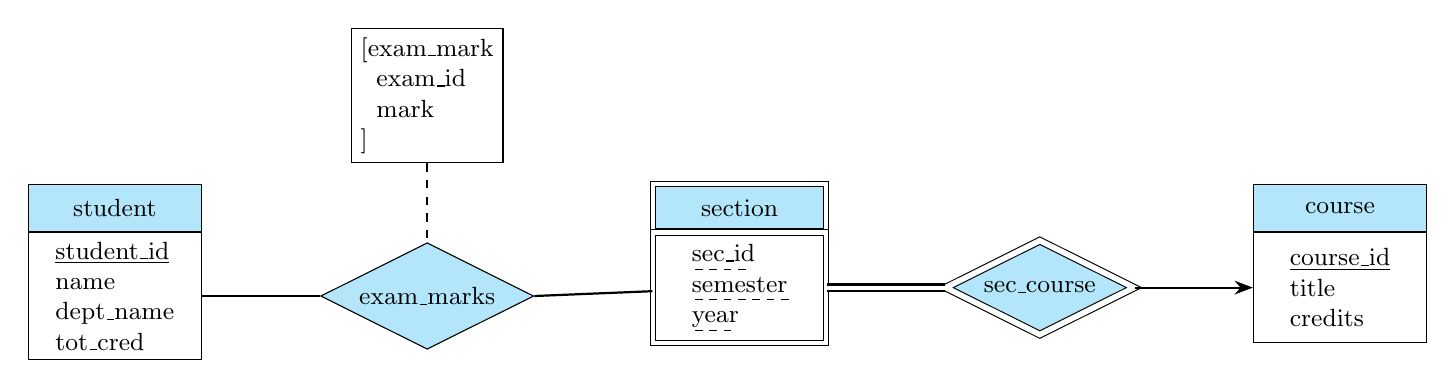
\begin{tikzpicture}[node distance=1.5cm]
    % Student table
    \node[box, fill=cyan!30, minimum height=0.6cm, minimum width=2.2cm] (student_header) {student};
    \node[box, fill=white, below=0cm of student_header.south, anchor=north, minimum height=1.4cm, minimum width=2.2cm] (student_body) {\underline{student\_id}\\name\\dept\_name\\tot\_cred};

    % Exam Marks clarifying table
    \node[decision, fill=cyan!30, right=1.5cm of student_body, inner sep=0.09cm] (check) {exam\_marks};

    % Exam Marks Diamond
    \node[box, above=1cm of check] (exam) {[exam\_mark\\\hspace{0.2cm}exam\_id\\\hspace{0.2cm}mark\\]};
    
    % Section table
    \node[doublebox, fill=cyan!30, minimum height=0.6cm, minimum width=2.2cm, right=1.5cm of check] (section_header) at (check.east |- student_header) {section};
    \node[doublebox, fill=white, below=0cm of section_header.south, anchor=north, minimum height=1.4cm, minimum width=2.2cm] (section_body) {\dashuline{sec\_id}\\\dashuline{semester}\\\dashuline{year}};

    % Sec Course Diamond
    \node[doubledecision, fill=cyan!30, right=1.5cm of section_body, double distance=2pt] (check2) {sec\_course};
    
    % Course table
    \node[box, fill=cyan!30, minimum height=0.6cm, minimum width=2.2cm, right=1.5cm of check2] (course_header) at (check2.east |- student_header) {course};
    \node[box, fill=white, below=0cm of course_header.south, anchor=north, minimum height=1.4cm, minimum width=2.2cm] (course_body) {\underline{course\_id}\\title\\credits};
    
    % Arrows
    \draw[line] (student_body) -- (check);
    \draw[dashedline] (exam) -- (check);
    \draw[line] (check.east) -- (section_body);
    \draw[doubleline] (section_body) -- (check2);
    \draw[arrow] (check2) -- (course_body); 
\end{tikzpicture}\vspace{1em}
\end{center}
\begin{checkboxes}
    \CorrectChoice 4
    \choice 5
    \choice 3
    \choice 2
\end{checkboxes}
\end{minipage}\vspace{1em}

\begin{minipage}{\linewidth}
\question[2]
What is the name of an attribute, in an E-R Diagram, whose value can be calculated on the basis of the values of other attributes?\par\vspace{0.5em}
\begin{checkboxes}
    \choice simple
    \choice composite
    \choice multivalued
    \CorrectChoice derived
\end{checkboxes}
\end{minipage}\vspace{1em}

\begin{minipage}{\linewidth}
\question[4]
What is the \textit{best} way to reduce the following subset of an ERD to a set of relations?\par\vspace{0.5em}
\begin{center}
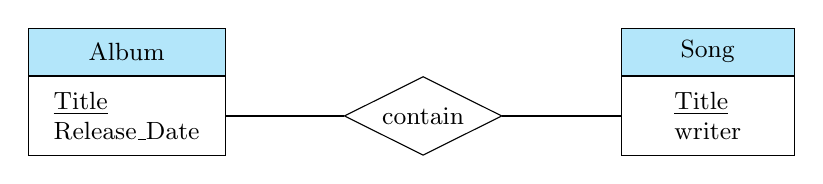
\begin{tikzpicture}[node distance=1.5cm]
    % Album table
    \node[box, fill=cyan!30, minimum height=0.6cm, minimum width=2.5cm] (album_header) {Album};
    \node[box, fill=white, below=0cm of album_header.south, anchor=north, minimum height=1cm, minimum width=2.5cm] (album_body) {\underline{Title}\\Release\_Date};

    % Contain diamond
    \node[decision, right=1.5cm of album_body, inner sep=0.09cm] (contain) {contain};
    
    % Song table
    \node[box, fill=cyan!30, minimum height=0.6cm, minimum width=2.2cm, right=1.5cm of contain] (song_header) at (contain.east |- album_header) {Song};
    \node[box, fill=white, below=0cm of song_header.south, anchor=north, minimum height=1cm, minimum width=2.2cm] (song_body) {\underline{Title}\\writer};
    
    % Lines
    \draw[line] (album_body) -- (contain);
    \draw[line] (contain) -- (song_body);
\end{tikzpicture}\vspace{1em}
\end{center}
\begin{checkboxes}
    \choice \textit{Album(\underline{Album\_Title}, Release\_Date)}\\\textit{Song(\underline{Album\_Title}, \underline{Song\_Title}, writer)}
    \CorrectChoice \textit{Album(\underline{Album\_Title}, Release\_Date)}\\\textit{Song(\underline{Song\_Title}, writer)}\\\textit{Song\_Album(\underline{Album\_Title}, \underline{Song\_Title})}
    \choice \textit{Album(\underline{Album\_Title}, Release\_Date, \underline{Song\_Title}, writer)}
    \choice \textit{Album(\underline{Album\_Title}, Release\_Date)}\\\textit{Song(\underline{Album\_Title}, Song\_Title, writer)}
    \choice \textit{Album(\underline{Album\_Title}, Song\_Title, Release\_Date)}\\\textit{Song(\underline{Song\_Title}, writer)}
\end{checkboxes}
\end{minipage}\vspace{1em}

% ------------------ MULTIPLE SELECT SECTION ------------------
\section*{Part III — Multiple select (select all that apply)}

\begin{minipage}{\linewidth}
\question[16]
What is true about the below diagram?\par
(Select all that apply.)\par\vspace{1em}
\begin{center}
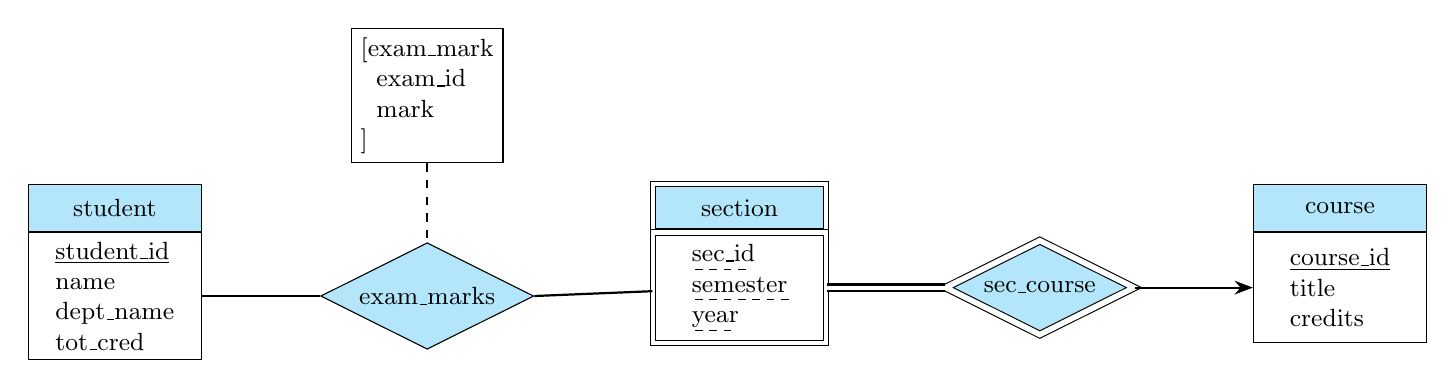
\begin{tikzpicture}[node distance=1.5cm]
    % Student table
    \node[box, fill=cyan!30, minimum height=0.6cm, minimum width=2.2cm] (student_header) {student};
    \node[box, fill=white, below=0cm of student_header.south, anchor=north, minimum height=1.4cm, minimum width=2.2cm] (student_body) {\underline{student\_id}\\name\\dept\_name\\tot\_cred};

    % Exam Marks clarifying table
    \node[decision, fill=cyan!30, right=1.5cm of student_body, inner sep=0.09cm] (check) {exam\_marks};

    % Exam Marks Diamond
    \node[box, above=1cm of check] (exam) {[exam\_mark\\\hspace{0.2cm}exam\_id\\\hspace{0.2cm}mark\\]};
    
    % Section table
    \node[doublebox, fill=cyan!30, minimum height=0.6cm, minimum width=2.2cm, right=1.5cm of check] (section_header) at (check.east |- student_header) {section};
    \node[doublebox, fill=white, below=0cm of section_header.south, anchor=north, minimum height=1.4cm, minimum width=2.2cm] (section_body) {\dashuline{sec\_id}\\\dashuline{semester}\\\dashuline{year}};

    % Sec Course Diamond
    \node[doubledecision, fill=cyan!30, right=1.5cm of section_body, double distance=2pt] (check2) {sec\_course};
    
    % Course table
    \node[box, fill=cyan!30, minimum height=0.6cm, minimum width=2.2cm, right=1.5cm of check2] (course_header) at (check2.east |- student_header) {course};
    \node[box, fill=white, below=0cm of course_header.south, anchor=north, minimum height=1.4cm, minimum width=2.2cm] (course_body) {\underline{course\_id}\\title\\credits};
    
    % Arrows
    \draw[line] (student_body) -- (check);
    \draw[dashedline] (exam) -- (check);
    \draw[line] (check.east) -- (section_body);
    \draw[doubleline] (section_body) -- (check2);
    \draw[arrow] (check2) -- (course_body); 
\end{tikzpicture}\vspace{1em}
\end{center}
\begin{checkboxes}
    \CorrectChoice There is one multivalued attribute.
    \choice There is one derived attribute.
    \CorrectChoice Every object of type \textit{section} is associated with exactly one object of type \textit{course}.
    \CorrectChoice \textit{sec\_id} doesn't uniquely identify a section.
    \CorrectChoice There may be no sections for a course.
    \CorrectChoice Grades that students get in different exams of different course offerings (sections) are recorded in the database.
    \choice One relationship is of type one-to-one
    \choice Student has to receive at least one grade for some test of a course section.
\end{checkboxes}
\end{minipage}\vspace{1em}

\begin{minipage}{\linewidth}
\question[4]
Choose triggering events.\par
(Select all that apply)\par\vspace{0.5em}
\begin{checkboxes}
    \CorrectChoice update
    \CorrectChoice insert
    \choice create
    \CorrectChoice delete
\end{checkboxes}
%---\begin{solution}
%--- format for giving solution descriptions
%---\end{solution}
\end{minipage}\vspace{1em}

\begin{minipage}{\linewidth}
\question[8]
Which statements, if any, are true about the below trigger?\par\vspace{0.5em}
\begin{verbatim}
create trigger t1 
before update on takes
for each row
begin
  if (new.grade = '')
  then set new.grade = null;
  end if;
end
\end{verbatim}
(Select all that apply)\par\vspace{0.5em}
\begin{checkboxes}
    \choice It ensures the grades are not equal to an empty string ('').
    \choice It doesn't work because there is no access to the variable new in the trigger with condition "\textbf{before update}"
    \choice If the first occurrence of the variable new was replaced with the variable old, then the trigger would ensure the updated grade is not an empty string ('')
    \CorrectChoice None of the statements are true.
\end{checkboxes}
%---\begin{solution}
%--- format for giving solution descriptions
%---\end{solution}
\end{minipage}\vspace{1em}

\begin{minipage}{\linewidth}
\question[12]
What is true about the below diagram?\par\vspace{0.5em}
\begin{center}
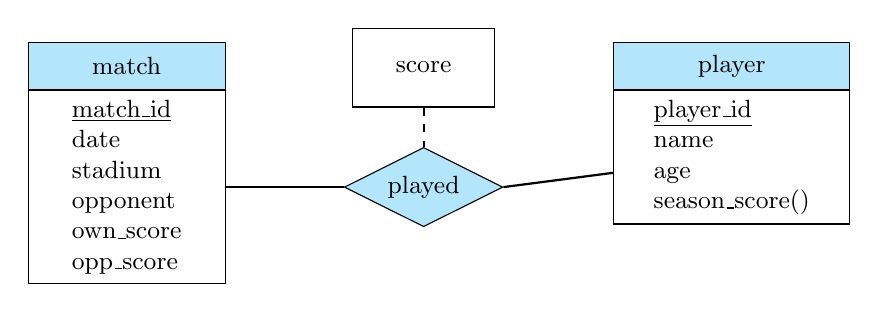
\begin{tikzpicture}[node distance=1.5cm]
    % match table
    \node[box, fill=cyan!30, minimum height=0.6cm, minimum width=2.5cm] (match_header) {match};
    \node[box, fill=white, below=0cm of match_header.south, anchor=north, minimum height=1cm, minimum width=2.5cm] (match_body) {\underline{match\_id}\\date\\stadium\\opponent\\own\_score\\opp\_score};

    % played diamond
    \node[decision, fill=cyan!30, right=1.5cm of match_body, inner sep=0.09cm] (played) {played};

    % Score box
    \node[box, fill=white, above=0.5cm of played] (score) {score};

    % player table
    \node[box, fill=cyan!30, minimum height=0.6cm, minimum width=3cm, right=1.5cm of score] (player_header) at (score.east |- match_header) {player};
    \node[box, fill=white, below=0cm of player_header.south, anchor=north, minimum height=1cm, minimum width=3cm] (player_body) {\underline{player\_id}\\name\\age\\season\_score()};
    
    % Lines
    \draw[line] (match_body) -- (played);
    \draw[dashedline] (score) -- (played);
    \draw[line] (played.east) -- (player_body);
\end{tikzpicture}\vspace{1em}
\end{center}
(Select all that apply)\par\vspace{0.5em}
\begin{checkboxes}
    \CorrectChoice Table \textit{player} will have 3 attributes in the database.
    \CorrectChoice There will be two foreign keys in the database in some table(s)
    \choice At least one player needs to play in a match.
    \CorrectChoice \textit{player\_id} uniquely identifies a player
\end{checkboxes}
%---\begin{solution}
%--- format for giving solution descriptions
%---\end{solution}
\end{minipage}\vspace{1em}

\begin{minipage}{\linewidth}
\question[18]
What is true about the below diagram?\par
(Select all that apply.)\par\vspace{1em}
\begin{center}
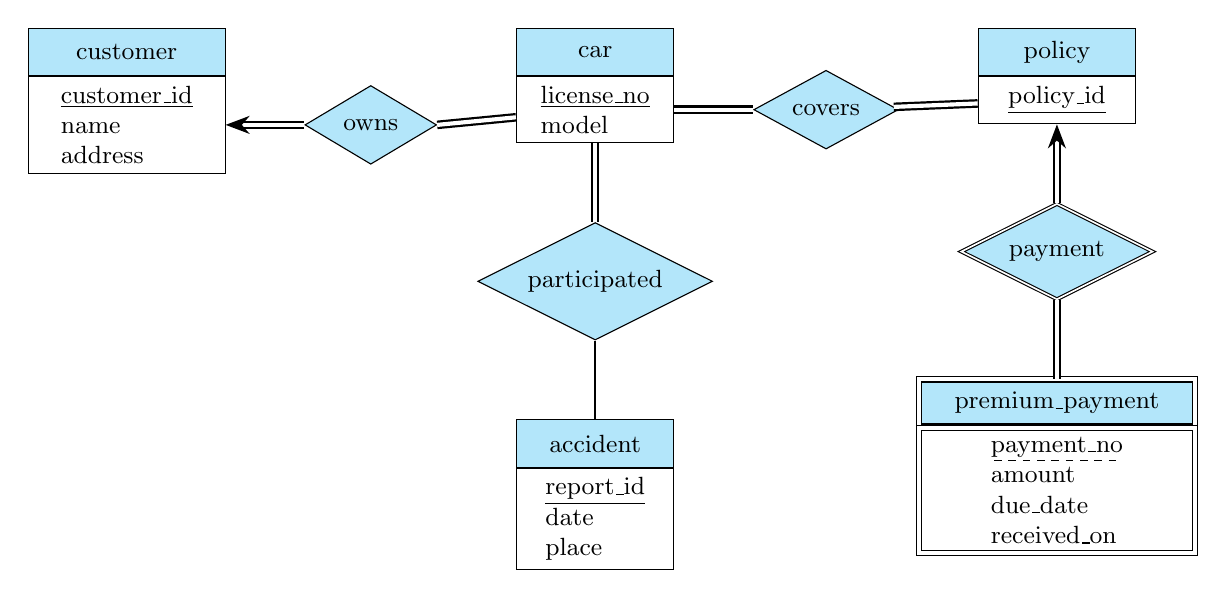
\begin{tikzpicture}[node distance=2cm]
    % Customer table
    \node[box, fill=cyan!30, minimum height=0.6cm, minimum width=2.5cm] (customer_header) {customer};
    \node[box, fill=white, below=0cm of customer_header.south, anchor=north, minimum height=1.2cm, minimum width=2.5cm] (customer_body) {\underline{customer\_id}\\name\\address};
    
    % Owns diamond
    \node[decision, fill=cyan!30, right=1cm of customer_body] (owns) {owns};
    
    % Car table
    \node[box, fill=cyan!30, minimum height=0.6cm, minimum width=2cm, right=1cm of owns] (car_header) at (owns.east |- customer_header) {car};
    \node[box, fill=white, below=0cm of car_header.south, anchor=north, minimum height=0.8cm, minimum width=2cm] (car_body) {\underline{license\_no}\\model};
    
    % Covers diamond
    \node[decision, fill=cyan!30, right=1cm of car_body] (covers) {covers};
    
    % Policy table
    \node[box, fill=cyan!30, minimum height=0.6cm, minimum width=2cm, right=1cm of covers] (policy_header) at (covers.east |- car_header) {policy};
    \node[box, fill=white, below=0cm of policy_header.south, anchor=north, minimum height=0.6cm, minimum width=2cm] (policy_body) {\underline{policy\_id}};
    
    % Participated diamond
    \node[decision, fill=cyan!30, below=1cm of car_body] (participated) {participated};
    
    % Accident table
    \node[box, fill=cyan!30, minimum height=0.6cm, minimum width=2cm, below=1cm of participated] (accident_header) {accident};
    \node[box, fill=white, below=0cm of accident_header.south, anchor=north, minimum height=1.2cm, minimum width=2cm] (accident_body) {\underline{report\_id}\\date\\place};
    
    % Payment diamond (double border)
    \node[doubledecision, fill=cyan!30, below=1cm of policy_body] (payment) {payment};
    
    % Premium_payment table (double border)
    \node[doublebox, fill=cyan!30, minimum height=0.6cm, minimum width=3.5cm, below=1cm of payment] (premium_header) {premium\_payment};
    \node[doublebox, fill=white, below=0cm of premium_header.south, anchor=north, minimum height=1.4cm, minimum width=3.5cm] (premium_body) {\dashuline{payment\_no}\\amount\\due\_date\\received\_on};
    
    % Lines and arrows
    \draw[doublearrow] (owns) -- (customer_body);
    \draw[doubleline] (owns.east) -- (car_body);
    \draw[doubleline] (car_body) -- (covers);
    \draw[doubleline] (covers) -- (policy_body);
    \draw[doubleline] (car_body) -- (participated);
    \draw[line] (participated) -- (accident_header);
    \draw[doublearrow] (payment) -- (policy_body);
    \draw[doubleline] (payment) -- (premium_header);
    
\end{tikzpicture}
\end{center}
\begin{checkboxes}
    \CorrectChoice Car has to participate in at least one accident.
    \CorrectChoice Policy covers one or more cars and car is covered by at least one policy.
    \choice A car can have many owners.
    \choice 8 tables will be created in the database.
    \choice \textit{premium\_payment} table will have two primary keys in the database
    \CorrectChoice There can be more than one tuple with value 1 for the attribute \textit{payment\_no} in the database
\end{checkboxes}
\end{minipage}\vspace{1em}

% ------------------ Fill In The Blank SECTION ------------------
\section*{Part IV — Fill In The Blank}

\begin{minipage}{\linewidth}
\question[2]
An entity whose existence depends on another entity is called a \ifprintanswers\textbf{weak/dependent }\else\fillin[][8em]\fi entity.
\end{minipage}\vspace{1em}

\begin{minipage}{\linewidth}
\question[4]
Based on the "E-R Diagram for a University Enterprise" relation corresponding to the sec\_time\_slot relationship should have a primary key consisting of
 \ifprintanswers\textbf{7 }\else\fillin[][8em]\fi attributes.
\begin{solution}
\begin{verbatim}
course_id
sec_id
semester
year
time_slot_id
day
start_time

Attributes of the primary key of the course relation plus attributes of the primary key 
of the time_slot relation.
\end{verbatim}
\end{solution}
\end{minipage}\vspace{1em}

\begin{minipage}{\linewidth}
\question[10]
Construct an E-R diagram for a car insurance company whose customers own one or more cars and no two customers own the same car. 
Customer is uniquely identified by a customer number. Each car has associated with it zero to any number of recorded accidents. 
Car is uniquely identified by a car number. An accident may be associated with 1 or more cars and is assigned unique identifier. 
Each insurance policy, identified uniquely by policy number, covers one or more cars and has one or more premium payments associated with it. 
Each payment, uniquely identified within the context of the policy, is associated with a specific period and has a due date. 
Additionally, the payment information includes the date on which the payment was received. 
There are \ifprintanswers\textbf{\_4\_ }\else\fillin[][8em]\fi strong entities and \ifprintanswers\textbf{\_1\_ }\else\fillin[][8em]\fi
weak entity set(s). There are \ifprintanswers\textbf{\_4\_ }\else\fillin[][8em]\fi relationships. 
The relationship between CAR entity and ACCIDENT entity is of type \ifprintanswers\textbf{many-to-many}\else\fillin[][8em]\fi. 
The relationship between entity CUSTOMER and entity CAR is of type \ifprintanswers\textbf{one-to-many/many-to-on}\else\fillin[][8em]\fi.
\end{minipage}\vspace{1em}

\end{questions}

\end{document}